\documentclass[a4paper]{report}
\usepackage{float}
\usepackage[utf8]{inputenc}
\usepackage[italian]{babel}
\usepackage{amsmath}
\usepackage{amssymb}
\usepackage{graphicx}
\graphicspath{ {./graph/} }
\usepackage{lmodern}
\usepackage{kpfonts}
\usepackage{titlesec}
\usepackage{listings}
\usepackage{color}
\usepackage{fontspec}
\usepackage{multirow}
\usepackage{float}
\usepackage{array}
\usepackage{afterpage}

\usepackage[font={small}, labelfont={bf}, format=hang, skip=8pt]{caption}

\setmainfont{Helvetica} % Set the main font to Helvetica
\setmonofont{Noto Sans Mono} % Set the monofont to Andale Mono

\definecolor{grigio}{rgb}{0.95,0.95,0.95}
\definecolor{mygrey}{rgb}{0.8,0.8,0.8}
\definecolor{mygreen}{rgb}{0.2,0.4,0.2}

\lstset{
  firstnumber=1,                % start line enumeration with line 1000
  language=Verilog,
  numbers=left,
  stepnumber=1,
  numbersep=4pt,
  numberstyle=\tiny\color{mygrey}, % the style that is used for the line-numbers
  backgroundcolor=\color{grigio},
  showspaces=false,
  showstringspaces=false,
  showtabs=false,
  tabsize=3,
  captionpos=b,
  breaklines=true,
  breakatwhitespace=true,
  escapeinside={\%*}{*)},
  basicstyle=\ttfamily\fontsize{8pt}{10pt}\selectfont, % Set the basic code style to a smaller font
  keywordstyle=\bfseries,
  commentstyle=\color{mygreen}
}

\titleformat{\chapter}[display]
{\normalfont\huge\bfseries\fontsize{14pt}{10pt}\selectfont}{\chaptertitlename\ \thechapter}{18pt}{\Huge}

\author{Tommi Bimbato VR500751, Antonio Iovine VR504083}
\title{Elaborato Assembly \\ \normalsize Corso di Architettura degli Elaboratori A.A. 2023/2024 \\ Prof.\ Franco Fummi, Prof.\ Michele Lora}

\begin{document}

\begin{titlepage}
  \maketitle
\end{titlepage}

\thispagestyle{empty} % Remove header from title page

\tableofcontents % Add table of contents

\begin{abstract}
  L'obiettivo del progetto è sviluppare un software per la pianificazione delle attività di un sistema produttivo. La produzione è organizzata in slot temporali uniformi, durante i quali un solo prodotto può essere in fase di lavorazione. Il software consentirà di ottimizzare la pianificazione delle attività secondo due algoritmi di pianificazioni differenti. L'intero software è stato sviluppato in linguaggio Assembly (Sintassi AT\&T) e testato su un insieme di dati di prova allegati a questa documentazione.
\end{abstract}

\chapter{Introduzione}
\section{Approccio progettuale}
L'elaborato è stato condotto seguendo un approccio metodologico strutturato. Inizialmente, è stata eseguita un'analisi dettagliata per identificare i requisiti e le funzionalità principali del software. Questo processo ha consentito una comprensione completa del contesto operativo e degli obiettivi da raggiungere.

Successivamente, è stata sviluppata una bozza del software utilizzando il linguaggio di programmazione C. Questo ha permesso la traduzione dei requisiti in una struttura logica e l'identificazione dell'architettura generale del software.

Parallelamente, sono stati definiti gli spazi di memoria necessari per la memorizzazione dei dati durante l'esecuzione del programma. Ciò ha garantito un utilizzo efficiente delle risorse disponibili.

Infine, sono stati eseguiti test approfonditi per verificare il corretto funzionamento del programma e identificare eventuali aree di miglioramento. L'iterazione su questo processo ha portato a modifiche e ottimizzazioni fino al raggiungimento di un livello soddisfacente di prestazioni e funzionalità.

\section{Analisi delle specifiche}
La produzione è organizzata in slot temporali uniformi, durante i quali un solo prodotto può essere in fase di lavorazione. Il programma analizza una serie di prodotti, ognuno caratterizzato da un identificativo, una durata, una scadenza e una priorità secondo le specifiche seguenti:
\begin{itemize}
  \item Identificativo: un codice da 1 a 127;
  \item Durata: il numero di slot temporali per il completamento (da 1 a 10);
  \item Scadenza: il limite massimo di tempo entro cui il prodotto deve essere completato (da 1 a 100);
  \item Priorità: un valore da 1 a 5, che indica sia la priorità che la penalità per il ritardo sulla scadenza\footnote{Il valore 5 indica la priorità più alta.}.
\end{itemize}
Al termine della pianificazione, il programma calcolerà la penale dovuta agli eventuali ritardi di produzione.

\subsection{Input}
L'utente invoca il programma "pianificatore" e fornisce due file come parametri da linea di comando, il primo viene considerato input, mentre il secondo viene utilizzato per salvare i risultati della pianificazione. Ad esempio:

\begin{verbatim}
pianificatore Ordini.txt Pianificazione.txt
\end{verbatim}

In questo caso, il programma caricherà gli ordini dal file \texttt{Ordini.txt} e salverà le statistiche stampate a video nel file \texttt{Pianificazione.txt}.

Se l'utente fornisce solo un parametro, il salvataggio della pianificazione su file verrà ignorato.

Il file degli ordini dovrà avere un prodotto per riga, con tutti i parametri separati da virgola. Ad esempio, se l'ordine fosse:
\begin{verbatim}
ID: 4; Durata: 10; Scadenza: 12; Priorità: 4;
\end{verbatim}
Il file dovrà contenere la seguente riga:
\begin{verbatim}
4,10,12,4
\end{verbatim}

\subsection{Algoritmi di pianificazione}
Una volta letto il file, il programma visualizzerà il menu principale, permettendo all'utente di selezionare l'algoritmo di pianificazione desiderato. Le opzioni disponibili sono:

\begin{enumerate}
  \item Earliest Deadline First (EDF): Si pianificano per primi i prodotti con scadenza più vicina. In caso di parità nella scadenza, si considera la priorità più alta.
  \item Highest Priority First (HPF): Si pianificano per primi i prodotti con la priorità più alta. In caso di parità di priorità, si considera la scadenza più vicina.
\end{enumerate}

L'utente può selezionare uno dei due algoritmi per la pianificazione delle attività del sistema produttivo.

\begin{figure}[H]
  \centering
  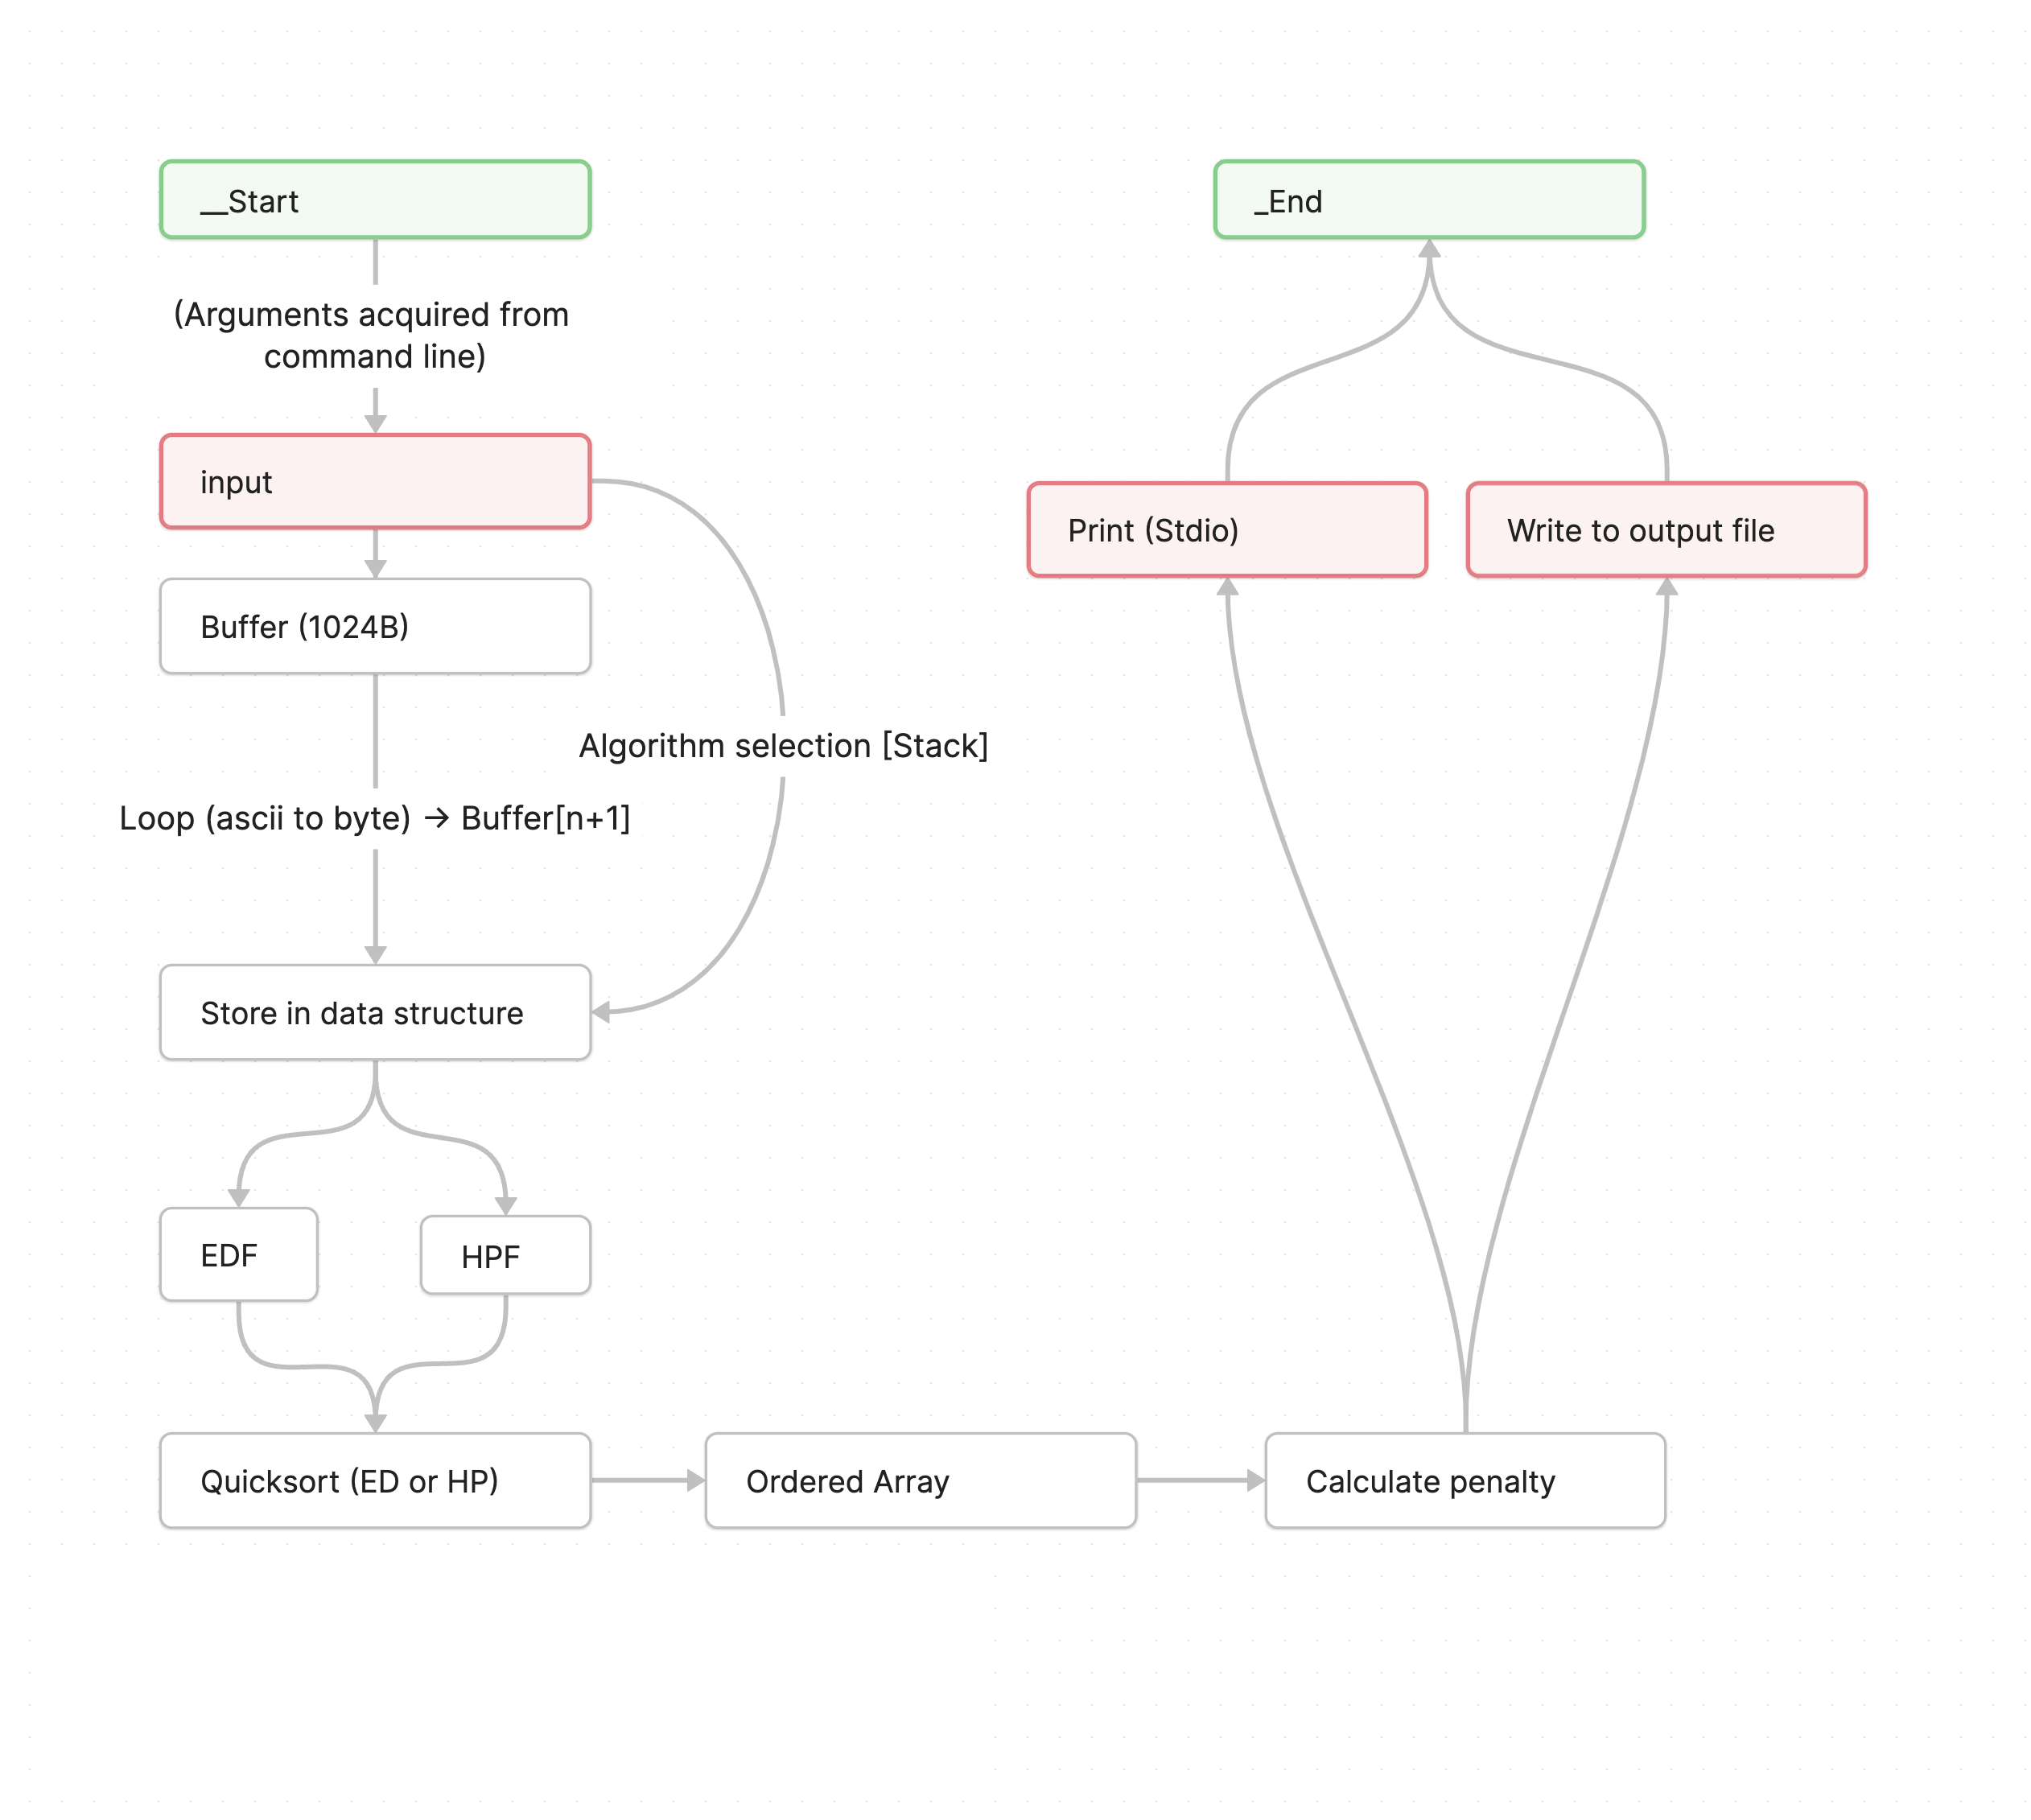
\includegraphics[width=\textwidth]{schema.png}
  \caption{Schema del sistema produttivo}
  \label{fig:schema}
\end{figure}

\subsection{Output}
Nel caso venisse specificato un file di output, il software stamperà su di esso i risultati della pianificazione secondo il seguente schema:
\begin{verbatim}
<Algoritmo di pianificazione scelto>:
<ID del prodotto>:<Inizio produzione>
[...]
Conclusione:<timeslot termine produzione>
Penalty:<penalità totale>
\end{verbatim}

\section{Funzionamento logico}

\subsection{Acquisizione e struttura dati}
Il software acquisisce l'intero contenuto del file di input e lo memorizza in una variabile nel buffer, parallelamente ne calcola la lunghezza (numero di righe) per allocare la memoria necessaria per la struttura dati vera e propria. Successivamente, il programma procede a leggere il contenuto del buffer, converte le informazioni dal formato ASCII al formato numerico e le memorizza in un array di struct. La peculiarità di questa struttura dati è che lo spazio occupato da un prodotto (ID, durata, scadenza e priorità) è di 4 byte totali, pari alla dimensione di un registro interno del processore considerato per l'applicazione del software.

\subsection{Ordinamento dei prodotti}
Acquisita la struttura dati, il programma acquisisce la scelta dell'algoritmo di pianificazione da parte dell'utente e procede con l'ordinamento dei prodotti in base alla scelta effettuata.

\subsection{Sorting}
Quick sort!

\subsection{Calcolo penali, salvataggio risultato ed uscita}
fprintf

\section{Codice}

...

\begin{lstlisting}[firstnumber=34]
  Codice in ASM!!!
  int main pippo VOID !!!
  ; Gibberish Assembly Code
  mov eax, 0
  add ebx, eax
  sub ecx, ebx
  mul edx, ecx
  div esi, edx
  push eax
  pop ebx
  inc ecx
  dec edx
  jmp label
  label:
  nop
  cmp eax, ebx
  jne label
\end{lstlisting}

\end{document}
